\documentclass{standalone}
\usepackage{PhysicalChemistryNote}
\begin{document}
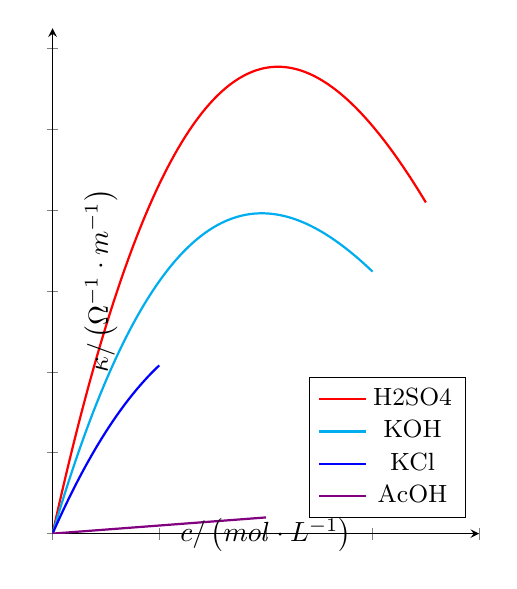
\begin{tikzpicture}
    \begin{axis}[
        width = 7cm,
        height = 8cm,
        legend pos = south east,
        xlabel = {$c/\left(\text{mol}\cdot\text{L}^{-1}\right)$},
        ylabel = {$\kappa/\left(\Omega^{-1}\cdot\text{m}^{-1}\right)$},
        axis lines = left,
        x label style={at={(axis description cs:0.5,0.05)},anchor=north},
        y label style={at={(axis description cs:0.175,0.5)},rotate=0,anchor=south},
        ymax = 1.25,
        ymin = 0,
        xmax = 0.8,
        ymin = 0,
        samples = 400,
        xticklabels={},
        yticklabels={}
    ]
    \addplot [thick, red, domain=0:0.7] {3*x*(x-1)*(x-2)};
    \addlegendentry{\small{\ce{H2SO4}}}
    \addplot [thick, cyan, domain=0:0.6] {3*x*(x-1)*(x-1.5)};
    \addlegendentry{\small{\ce{KOH}}}
    \addplot [thick, blue, domain=0:0.2] {2*x*(x-1)*(x-1.5)};
    \addlegendentry{\small{\ce{KCl}}}
    \addplot [thick, violet, domain=0:0.4] {0.1*x};
    \addlegendentry{\small{\ce{AcOH}}}
    \end{axis}
\end{tikzpicture}
\end{document}